\documentclass{bioinfo}
\copyrightyear{2015}
\pubyear{2015}

\begin{document}
\firstpage{1}

\title[short Title]{Pyveplot: SVG Hive Plot API}
\author[]{Rodrigo Garcia-Herrera}
\address{Department of Bioinformatics, National Institute of Genomic
  Medicine, Periferico Sur 4809, Mexico City 14610}

\history{Received on XXXXX; revised on XXXXX; accepted on XXXXX}

\editor{Associate Editor: XXXXXXX}

\maketitle

\begin{abstract}

\section{Sumary:}
Python package provides programmatic object oriented interface for the
creation of Hive plots in Scalable Vector Graphics format.
\section{Availability and Implementation:}
Freely available as a Python package at
https://pypi.python.org/pypi/pyveplot/

\section{Contact:} \href{rgarcia@inmegen.gob.mx}{rgarcia@inmegen.gob.mx}
\end{abstract}

\section{Introduction}

Hive plots (HPs) are a way of visualizing large networks which allow
for easy assesment and comparison of their structural properties.
\cite{krzywinski2012hive}

Although graphical user interfaces for the creation of HPs may be
easier to use or learn, an Application Programming Interface (API)
provides for more flexibility and automation which are boosted by the
use of a powerful programming language. Python is such a language:
mature and popular, it has a large number of libraries related to data
analysis in general and life sciences and bioinformatics in
particular. For example, it is easy to leverage the functionality
provided by the powerful NetworkX
library \cite{hagberg-2008-exploring}, while having no dependencies on
it.

Scalable Vector Graphics (SVG) is a modularized format for describing
two-dimensional vector graphics. It is based on XML and developed by
the World Wide Web Consortium \cite{McCormack:11:SVG}. While the
requirements of a HP can be met with the most basic shapes supported
by SVG, the design of Pyveplot allows a programmer to take full
advantage of the wide array of capabilities of the graphics format.

The design of the Pyveplot API favors a procedural, imperative way of
creating and linking the elements of a plot, at various degrees of
abstraction. For complex data this approach may have better
readability than e.g. declarative approaches, which obscure mecanisms in
favor of description of the wanted result.

\section{Object Oriented Approach}

The object oriented API makes the creation of a plot a straightforward
process. A HP consists of:
\begin{itemize}
\item radialy distributed linear axes
\item nodes along those axes
\item conections among those nodes
\end{itemize}
The API provides the corresponding objects: a {\bfseries Hiveplot} object
which contains an arbitrary number of {\bfseries Axis} objects which in
turn contain an arbitrary number of {\bfseries Node} objects, and a method
to connect them.

The ``Hiveplot.connect()'' method draws edges as bezier curves. Start
and end points are set when adding nodes to an axis with the
``Axis.add\_node()'' method, using the placement information of the
axis and a specified offset from its start point.

Control points are set at the same distance from the start (or end)
point of an axis as their corresponding nodes, but along an invisible
axis that shares its origin but diverges by a given angle.

The ``Drawing'' structural component of the underlying svgwrite
library (cite?) is available through the ``dwg'' (short for drawing)
property of {\bfseries Hiveplot}, {\bfseries Axis} and {\bfseries
  Node} objects. Any other shape or valid SVG element may be added to
them. This allows for a very flexible use of marks, tags, ticks, etc.,
as is shown in Figure \ref{fig:01}

More examples in repository: https://github.com/CSB-IG/pyveplot/


\begin{figure}
  \centerline{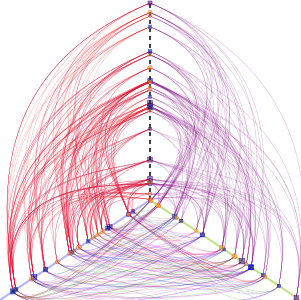
\includegraphics{example.png}}
  \caption{Hive plot of Erdos-Renyi graph trivially generated using
    NetworkX. Showing off some SVG goodness: paths that make edges
    and axes can have any width, color or dash pattern, any valid SVG
    element can be used as a node. Define as many axes as you need,
    place them anywhere in the SVG canvas.}
  \label{fig:01}
\end{figure}

\section*{Acknowledgement}
The author wishes to acknowledge the colaboration of the Computational and Systems
Biology/Integrative Genomics lab at INMEGEN.


\begin{thebibliography}{3}

\bibitem{krzywinski2012hive}
Martin Krzywinski, Inanc Birol, Steven~JM Jones, and Marco~A Marra.
\newblock Hive plots—rational approach to visualizing networks.
\newblock {\em Briefings in bioinformatics}, 13(5):627--644, 2012.


\bibitem{hagberg-2008-exploring}
Aric~A. Hagberg, Daniel~A. Schult, and Pieter~J. Swart.
\newblock Exploring network structure, dynamics, and function using {NetworkX}.
\newblock In {\em Proceedings of the 7th Python in Science Conference
  (SciPy2008)}, pages 11--15, Pasadena, CA USA, August 2008.


\bibitem{McCormack:11:SVG}
Cameron McCormack, Jonathan Watt, Doug Schepers, Anthony Grasso, Patrick
  Dengler, Jon Ferraiolo, Erik Dahlstr{\"{o}}m, Dean Jackson, Jun Fujisawa, and
  Chris Lilley.
\newblock Scalable vector graphics ({SVG}) {1.1} (second edition).
\newblock {W3C} recommendation, W3C, August 2011.
\newblock http://www.w3.org/TR/2011/REC-SVG11-20110816/.

\end{thebibliography}


\end{document}
